\chapter{The dataset}\label{cha:data}

This chapter introduces the dataset and work done to enable information extraction and analysis of the provided data. The case analyzed in the analysis is introduced. \todo{mention finding a case? not specified by hymatek}


% In the data set, there are three power plants that have pelton turbines with measurement of their needle position. More information about a pelton turbine can be found in chapter \ref{cha:data}. One of the power plants had recorded several issues with the control and behaviour of the needles during operation. There were many interesting events spread out over many of the power plants, but one major benefit with the pelton needle case, was that there was one plant with several reported issues for the same component. In most of the other cases, there were only recorded one incident on one plant, making them hard to analyze and validate. The fact that there also were two power plants in addition that had the same process signals without reported issues, opened up the possibility for testing and validating the chosen techniques not only on data from the faulty plant. This also introduced the possibility to validate how well and how easy the different techniques could adapt to new plants.    




% Based on the arguments above, the pelton needle case was chosen as the focus of the thesis. The following points were then defined as a basis for the analysis. 


\section{Dataset}\label{sec:dataset}
    Hymatek controls provided a dataset from a Norwegian energy company, containing process information from $27$ hydro electric powerplants logged from $2013$ to mid $2017$. The data is not pre-prosessed in any way, and come just as it is logged at the company. A big part of the thesis has been spent on exploring the data, finding out what is logged and what can be used. The data is split into five folders, one for each year. In each folder several different files are stored. Table \ref{tab:data_files} shows the different file types that are found in the dataset. The file names indicated the frequency, sampling type and sampling duration of the data. The files are not separated by plants, only by date. Hence, a file containing data sampled every second for any given start and stop date, contains data from all plants for that given period. In addition to the data files, a meta-data file is provided where plant name and process signal for each tag can be found.
    
    \begin{table}[]
        \centering
        \begin{tabular}{|c|c|c|c|c|}
            \hline
             Interval   & Average   & Max   & Min   & Actual    \\ \hline
             Daily      & x         & x     & x     & -         \\ \hline
             Hourly     & x         & x     & x     & -         \\ \hline
             Minutely   & x         & x     & x     & -         \\ \hline
             Secondly   & -         & -     & -     & x         \\ \hline
        \end{tabular}
        \caption{Table showing the available data for the different sampling frequencies}
        \label{tab:data_files}
    \end{table}
    
    The total size of all files exceeded $90$Gb, this means that one can't simply load all data into the computer memory, and work with it from there. The information needs to be extracted one plant at a time, for each of the different sampling rates, and stored in a way that enabled fast and efficient loading. All of the work with reading, processing and storing the data is done in python using the \textbf{Pandas} library. 
    
    
    
    \subsection{Old and new data format}\label{subsec:data_format}
        Regardless of sampling-rate and data type, the files are all on the same format. As seen in table \ref{tab:orig_data}, each line holds a tag, a time of sampling and a process value. 
        \begin{table}[h]
            \centering
            \begin{tabular}{|c c c|}
                \hline
                 Tag        & Timestamp         & Value  \\
                 192390514  & 20170101000000000 & 0.897244155 \\
                 192391514  & 20170101000000000 & -0.549806237 \\
                 \hline
            \end{tabular}
            \caption{Example of the structure of the original datasets}
            \label{tab:orig_data}
        \end{table}
        Once a file is loaded the tag is replaced by the process-signal name found in the meta-data file. To enable interpretation and analysis of the data, it is decided that new datasets needs to be created on the format shown in table \ref{tab:plant_format}.
        \begin{table}[h]
            \centering
            \begin{tabular}{|c|c|c|c|c|}
                \hline
                Time stamp & P. variable 1     & P. variable 2    & ..    & P. variable n    \\ \hline
                time 1        & NaN         & $2$           & ..    & NaN         \\ \hline
                time 2        & $3.00$      & NaN           & ..    & $0.00214$\\ \hline
            \end{tabular}
            \caption{Example showing how the data could look in the data format for each plant after reconstruction is complete}
            \label{tab:plant_format}
        \end{table}

        
    \subsection{Overview of the datasets}
        Once the data is reconstructed as specified in subsection \ref{subsec:data_format} one can look into what information it holds. The number of available process signals varies a lot, from above $250$ to below $20$, as can be seen in figure \ref{fig:process_signal_overview}. This is used as a first stage filtering to reduce the number of plants to examine. The plants with fewer than $30$ process-signals are dropped from the analysis, reducing the number of plants in the dataset to $15$.    
        
        \begin{figure}[h]
            \centering
            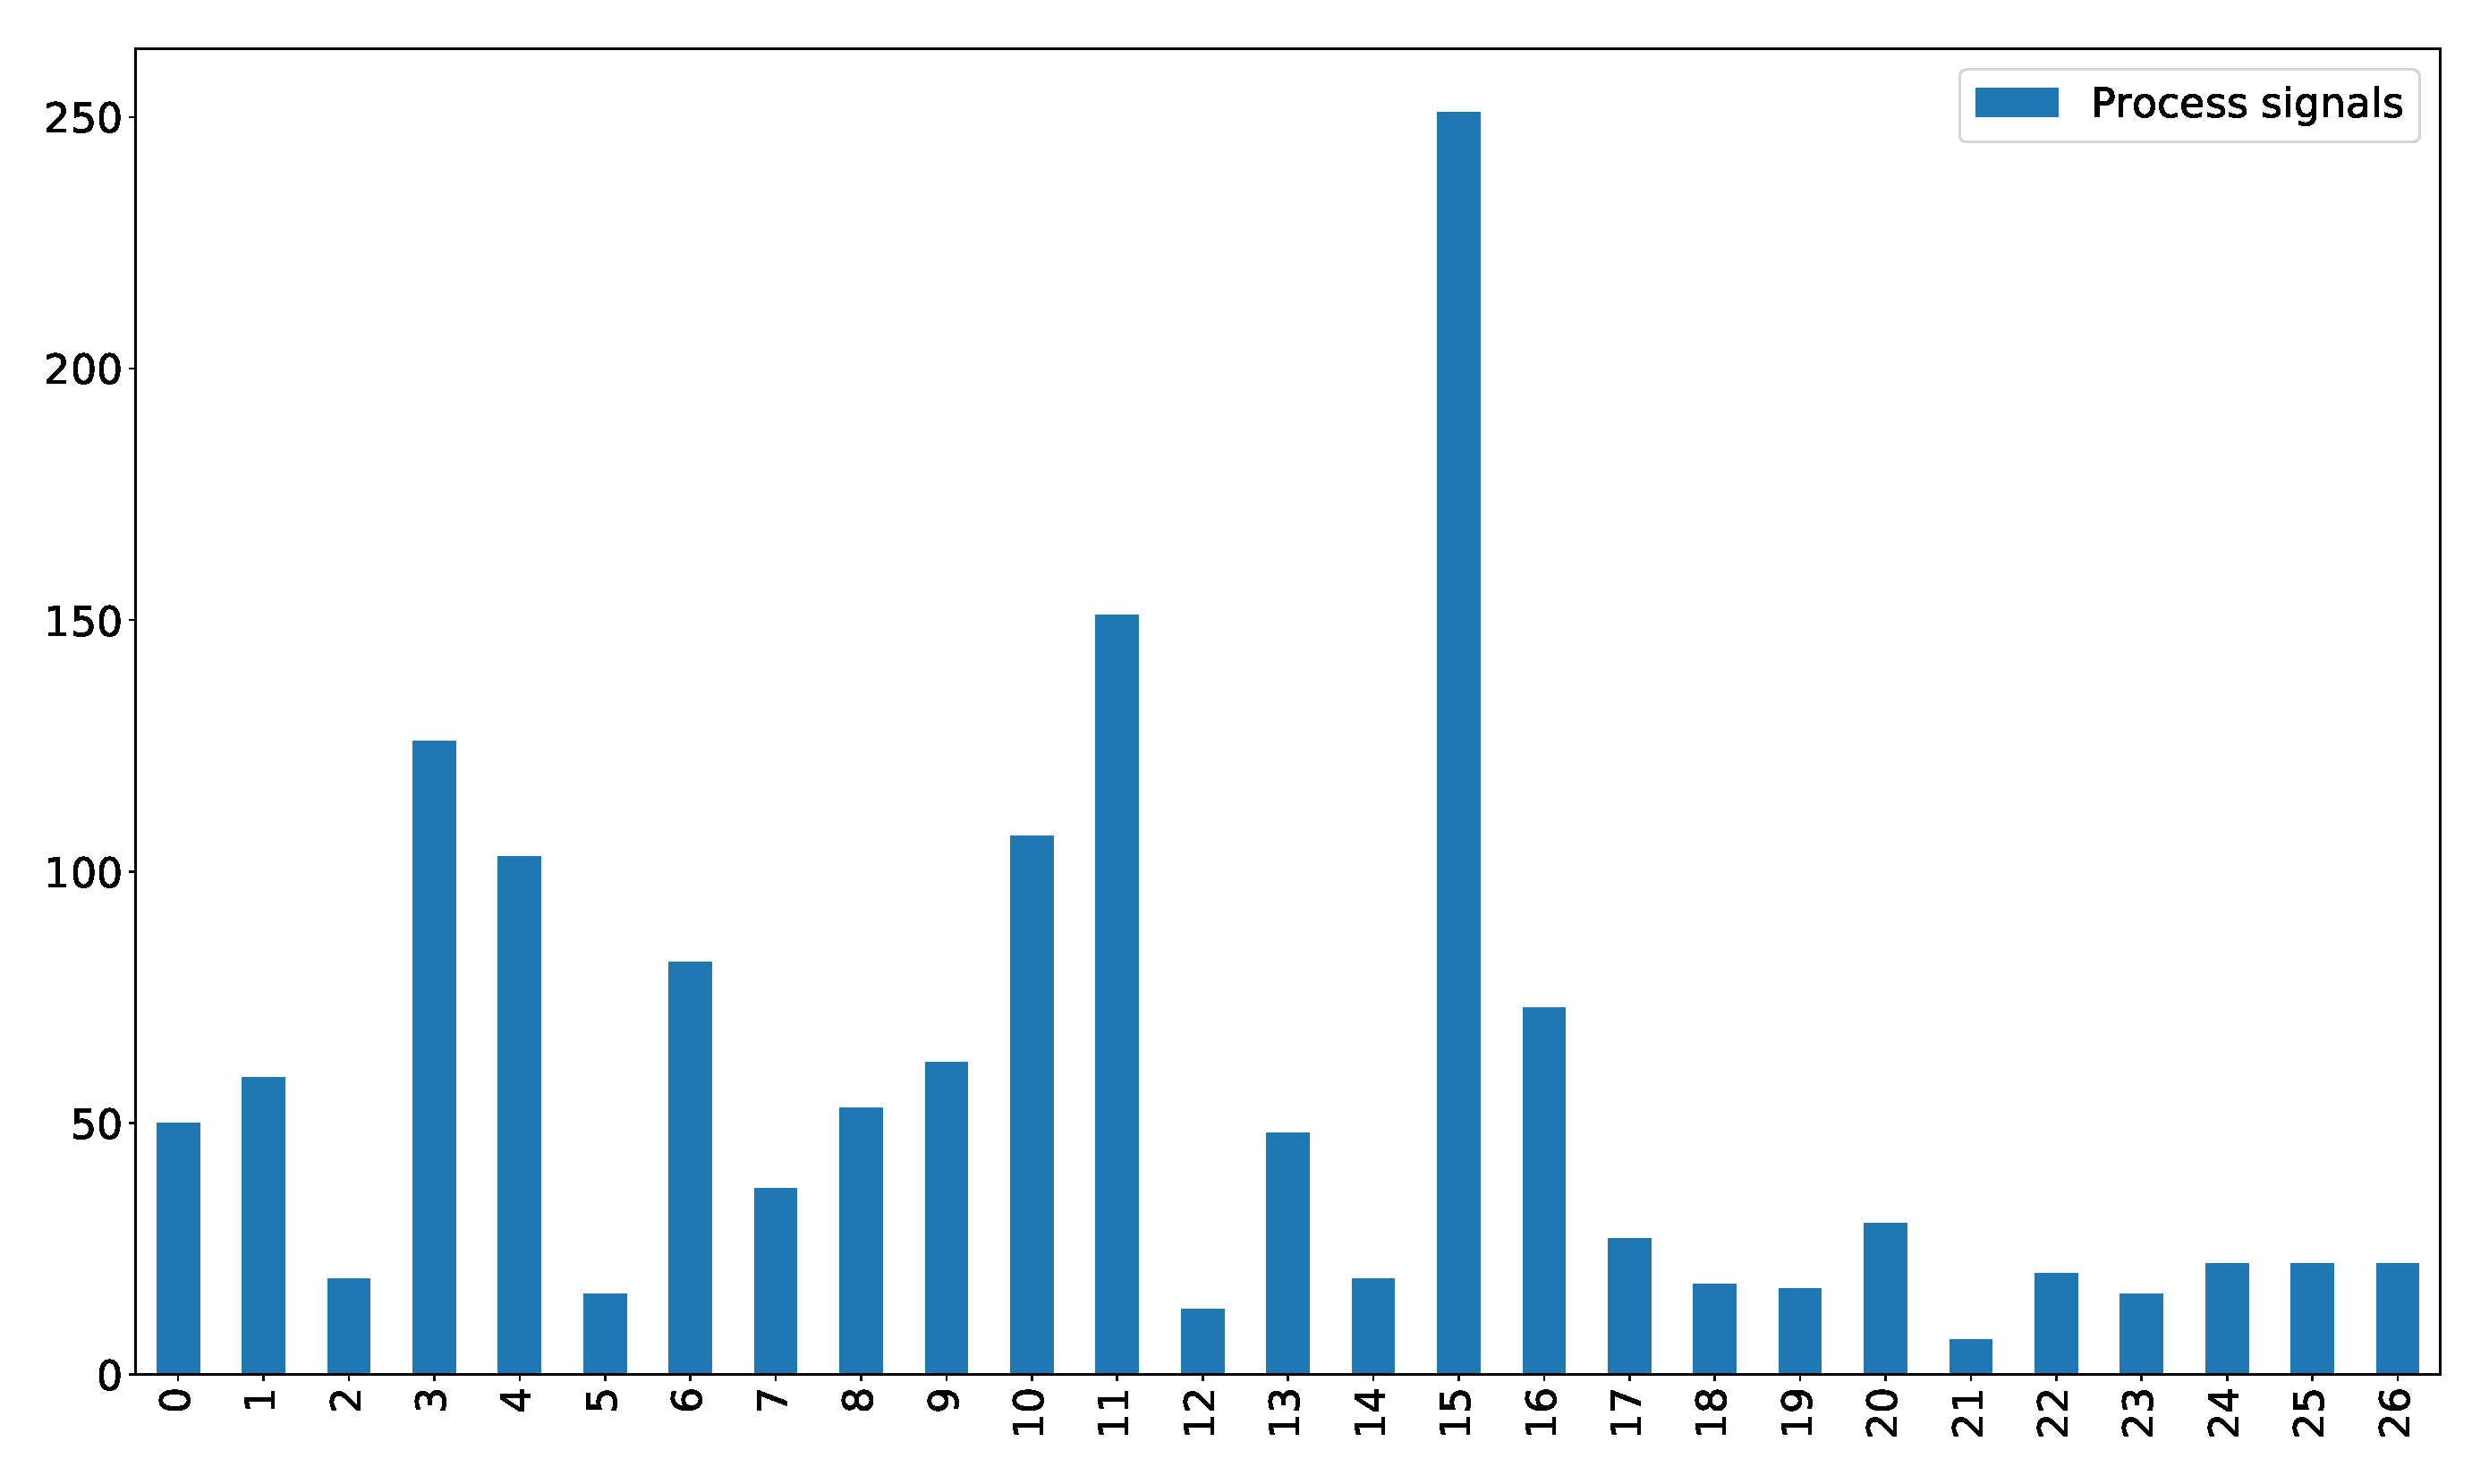
\includegraphics[width=\textwidth]{report/figures/data/plant_process_signals_overview.pdf}
            \caption{Overview of the number of process-signals for each of the 27 plants}
            \label{fig:process_signal_overview}
        \end{figure}
        
        After discarding the plants with few signals, the type of process-signals available are looked into. The more data sampled from different parts of a plant, the better. Having data from several parts and components of a plant can enable finding a link between unknown components and sensors. This can then be used to improve the knowledge of a plant beyond the pure measurements taken by each sensor. Figure \ref{fig:signal_type_overview} shows the different types of signals found in the datasets for the different plants. As can be seen temperature is one of the most common signals for all plants. There is also many signals of type "Def Type Måling", which is a common name that covers all signals not defined with its own tag. Pressure, level, vibration, etc are signals covered by this tag. Since all of the remaining plants had process-variables of different types, none are removed. 
        
        \begin{figure}
            \centering
            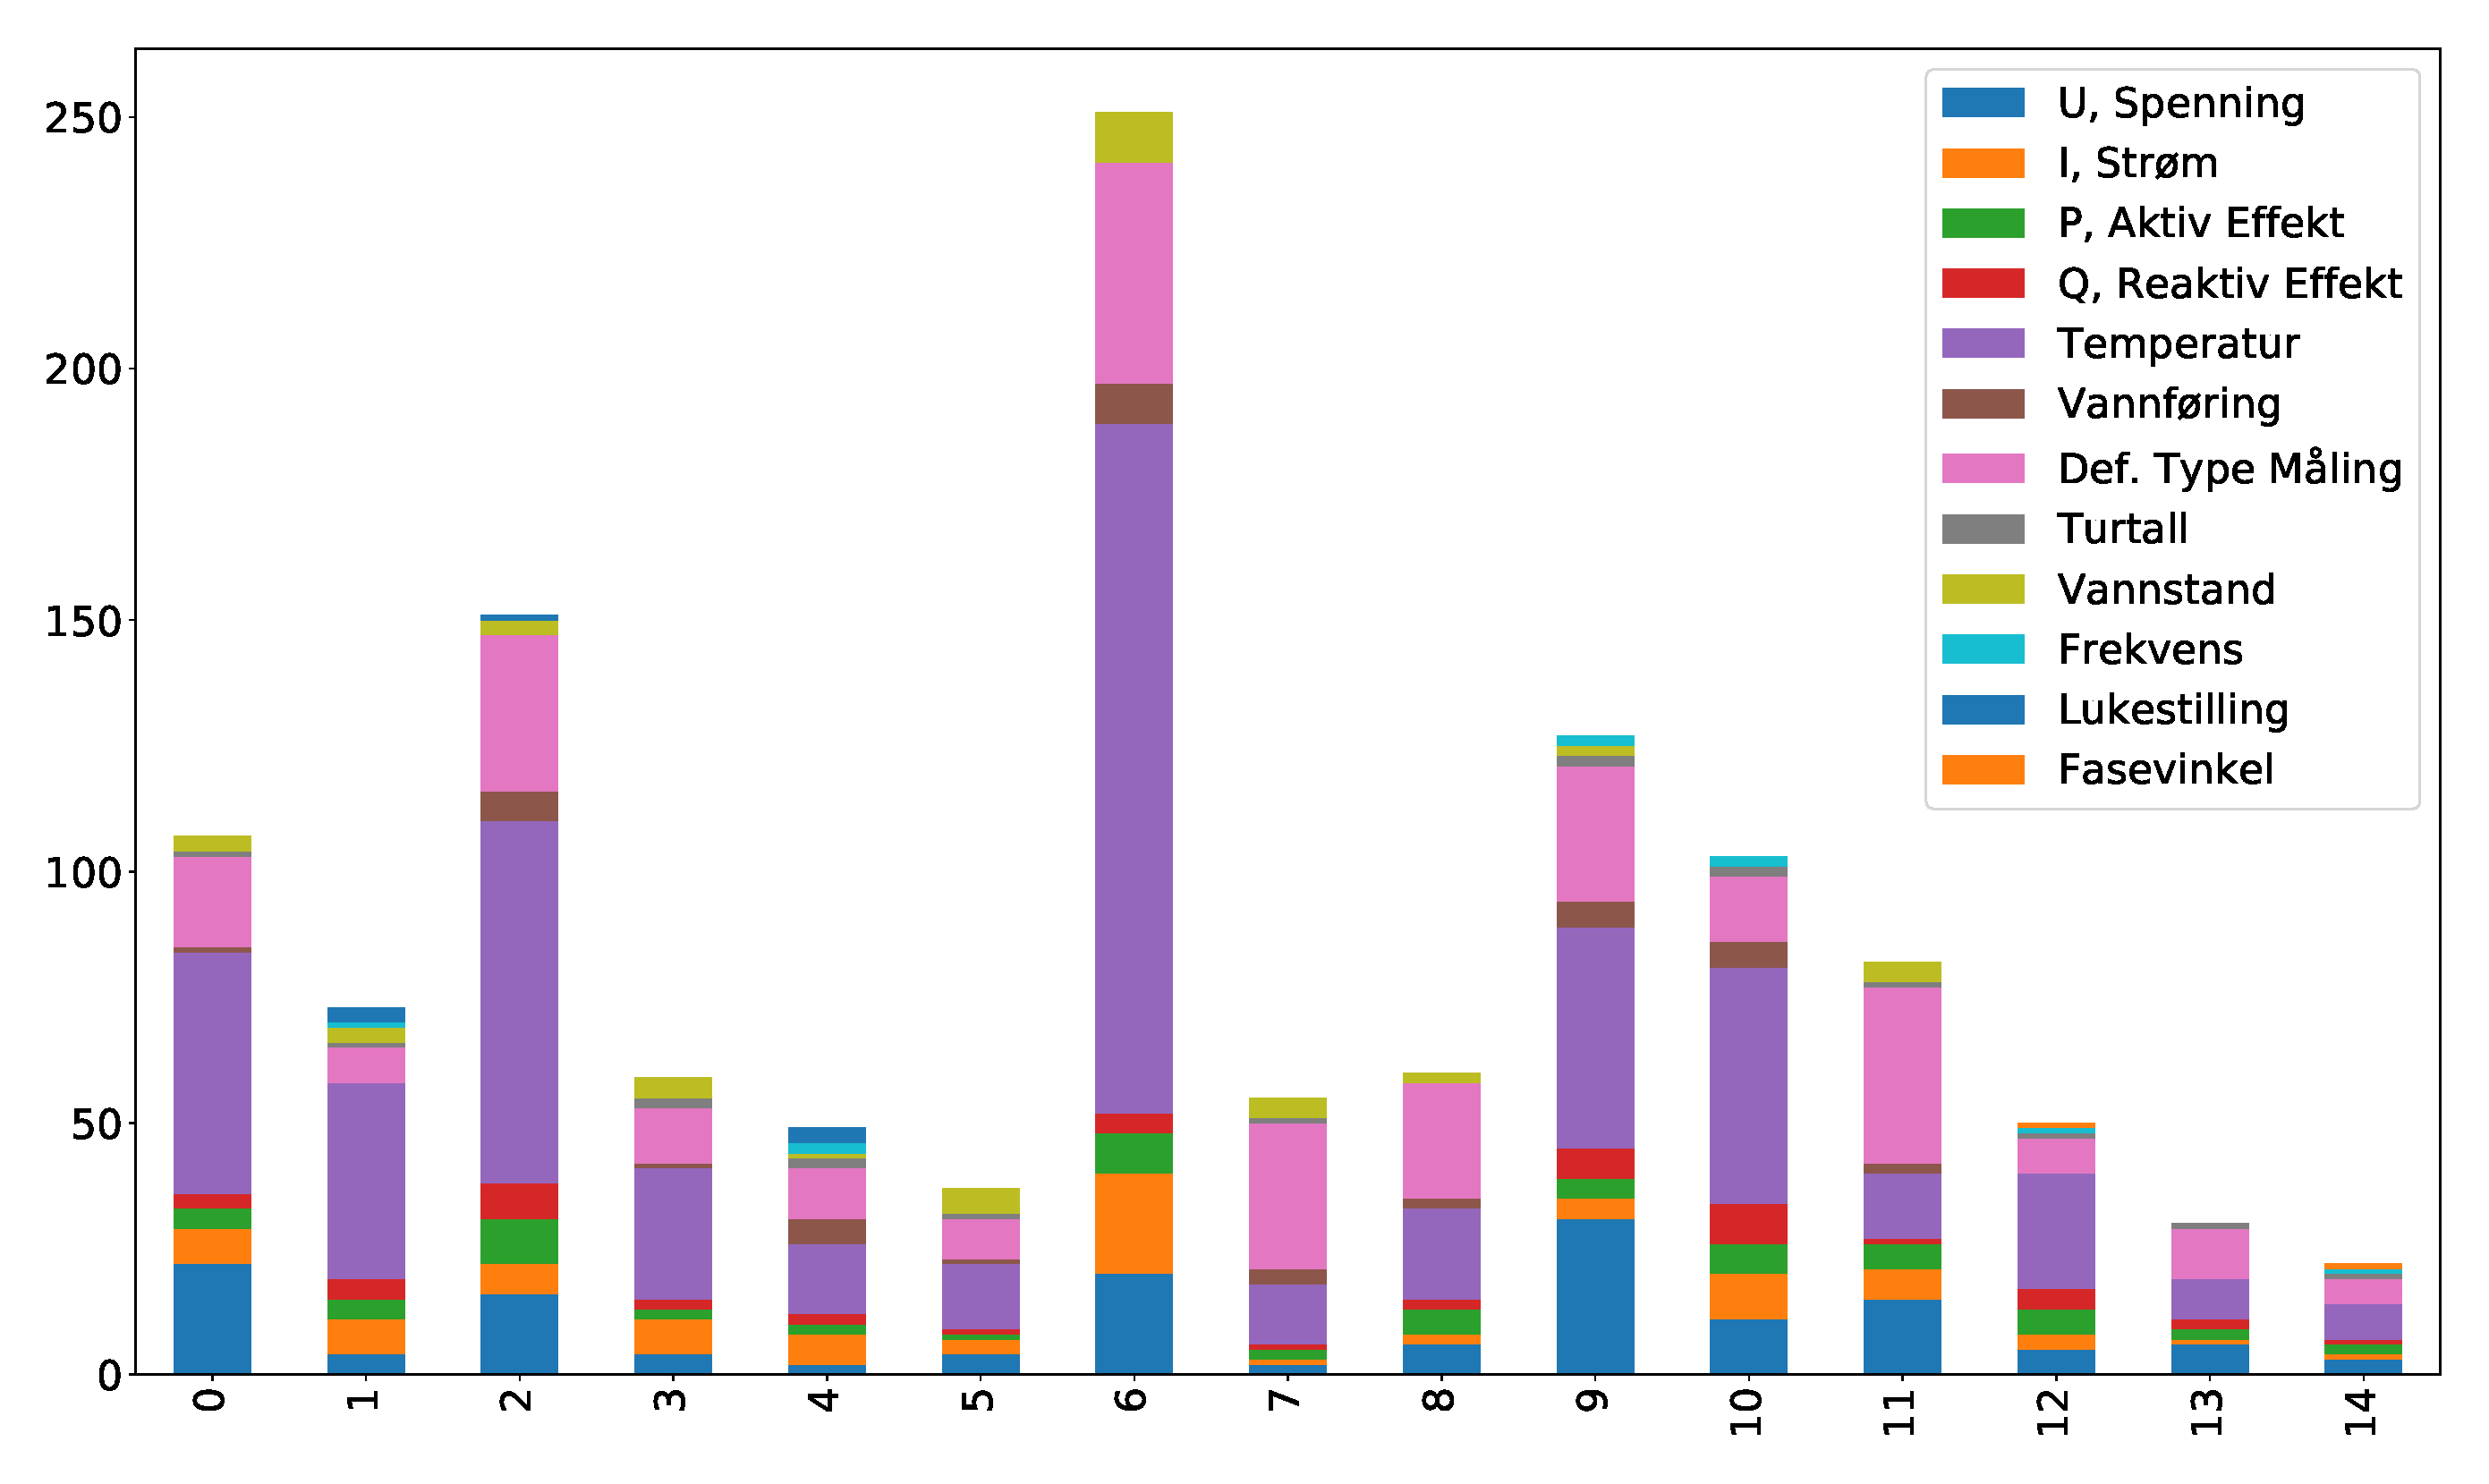
\includegraphics[width=\textwidth]{report/figures/data/plant_signal_types_overview.pdf}
            \caption{Figure showing the different variables found and the number of them in each plant dataset}
            \label{fig:signal_type_overview}
        \end{figure}
        
        % It is only necessary to keep the datasets with the highest sampling rate. The highest sampling rate will provide the most detail about a plant, and lower sampling rates can always be extracted from higher rates.
        
        % was decided to only use the datasets sampled every second. Using these datasets gave a snapshot of the plant state at a given time. Pandas has a lot of built in functionality that enables easy re-sampling, so that the average, max and min datasets could easily be recreated from this dataset if wanted.
        
        An issue arose when looking in detail at the datasets. Preferably, all process-signals should be sampled periodically and at the same time. This is however not the case, only at hourly resolution are the data matrices complete. At higher sampling rates there are a lot of missing data. At the highest sampling frequency (every second), there are many time-stamps where none of the process signals are sampled, and those that are sampled, often only samples one process-signal. This means that one either has to work with only hourly sample rate, work with incomplete datasets or reduce the number of process signals to investigate. Either the equipment used for sampling is not working as it should, or the varying sampling rate must be on purpose.\todo{add citation to the CM hydro paper with sampling scheme explained} This sheds light on the fact that having lots of data is not always a sign of quality. It is found that the data sampled in $2013$ is poorer than the later years, and hence it is dropped from any further analysis. 
    % \subsection{Instrumentation}\label{subsec:instrumentation}
    %     what is there of instrumentation? refer to the data I have gotten         
        
    \subsection{The historical log of the plants }
        Once an overview of the data was in place, the energy company was contacted, requesting an incident log from the remaining plants. Incident logs for the entire sampling period, for all of the $27$ power plants were received. The level of details in the logged incidents are very varying from plant to plant. Some plants have reported over 200 incidents, while others barely exceeded 20. Many of the incidents are also minor incidents like a broken light bulb or non functioning tools. This made finding interesting incidents time consuming. There were found several interesting incidents, but very few were reported to occur more than once. Having few incidents makes it hard to separate valuable information from noise. Only having a limited number of faults can easily lead to overfitting. There is always a risk that the correlations and variable dependencies found can be caused by randomness. This needs to be taken into consideration when working such cases.  
        
        In the log for one of the power plants it was found an error with the needles for a Pelton turbine. The error reported that as the opening of needle four of turbine two was decreased below $46\%$, it started to lag behind needle two. Checking the process variables from the plant, it was found that it has two turbines that both have four needles.\todo{remove this or add more analysis}When looking into the historical log of the plant, it was found that several more incidents with the Pelton needles were reported for the two turbines. A search through the $14$ remaining power plants, showed that there are two additional plants with Pelton turbines. One with four needles and one with five. These plants have however not reported any problems with the Pelton needles. This could then be a possible reference for normal operation, in addition it opens the possibility for testing how adaptable the anomaly detection methods are. 
        
\section{Pelton needles case}\label{sec:pelton_needles}
    The Pelton needle case was chosen for further analysis for several reasons. Firstly it is a critical part of the Pelton turbine, if the needles are not operating as they should it will affect the power produced by the turbine. The needle openings are a big part of a complex control-system, that controls that the turbine holds constant speed. If a method can be found that can give early warnings about incidents like the one above, maintenance can be planned and components can be overhauled before the system condition becomes so bad that it is no longer controllable. Secondly, having data from different plants makes it possible to analyze how well the methods and techniques used adapt to new data. This is an important factor, if one can develop a method that is transferable with little to no adaptation need between plants, the time for commissioning will be greatly reduced. In addition, this case fits well as a extension of my project thesis, where the condition of the guide vanes for a Francis turbine was analyzed. Finally, quality and available process variables varies a lot from plant to plant. One of the biggest issues was that the majority of the process signals were not sampled at a constant frequency. The Pelton needles were found to be sampled in a manner that allowed the use of data from two separate plants.
             

    \subsection{Pelton needle incident 02.03.2017}
        As the incident reported that one needle was lagging behind another, it could indicate pairwise operated needles. This can also be justified from a practical perspective, if the needles are placed opposite of each other they will give the turbine an even momentum as long as they lead the same amount of water onto the turbine. To confirm this, scatter-plots were created where each needle is plotted against the other. To enable this the needle process signals are pairwise extracted from the rest of the dataset, and all time-stamps where both needles are not sampled are removed. Figure \ref{fig:plant1_needles} shows the scatter-plot of the pairwise operated needles for both turbines at plant 1. As can be seen in all four plots, the majority of the data follows a linear dependency between the needles. However, there is clearly several data-points that deviate from this, especially for needle pair $[2,4]$ on turbine $2$. The plot in the bottom right corner shows what appears to be operational problems. It is only needle [1,3] on turbine one seen in the upper left plot, that follows the linear pattern.
        \begin{figure}[h]
            \centering
            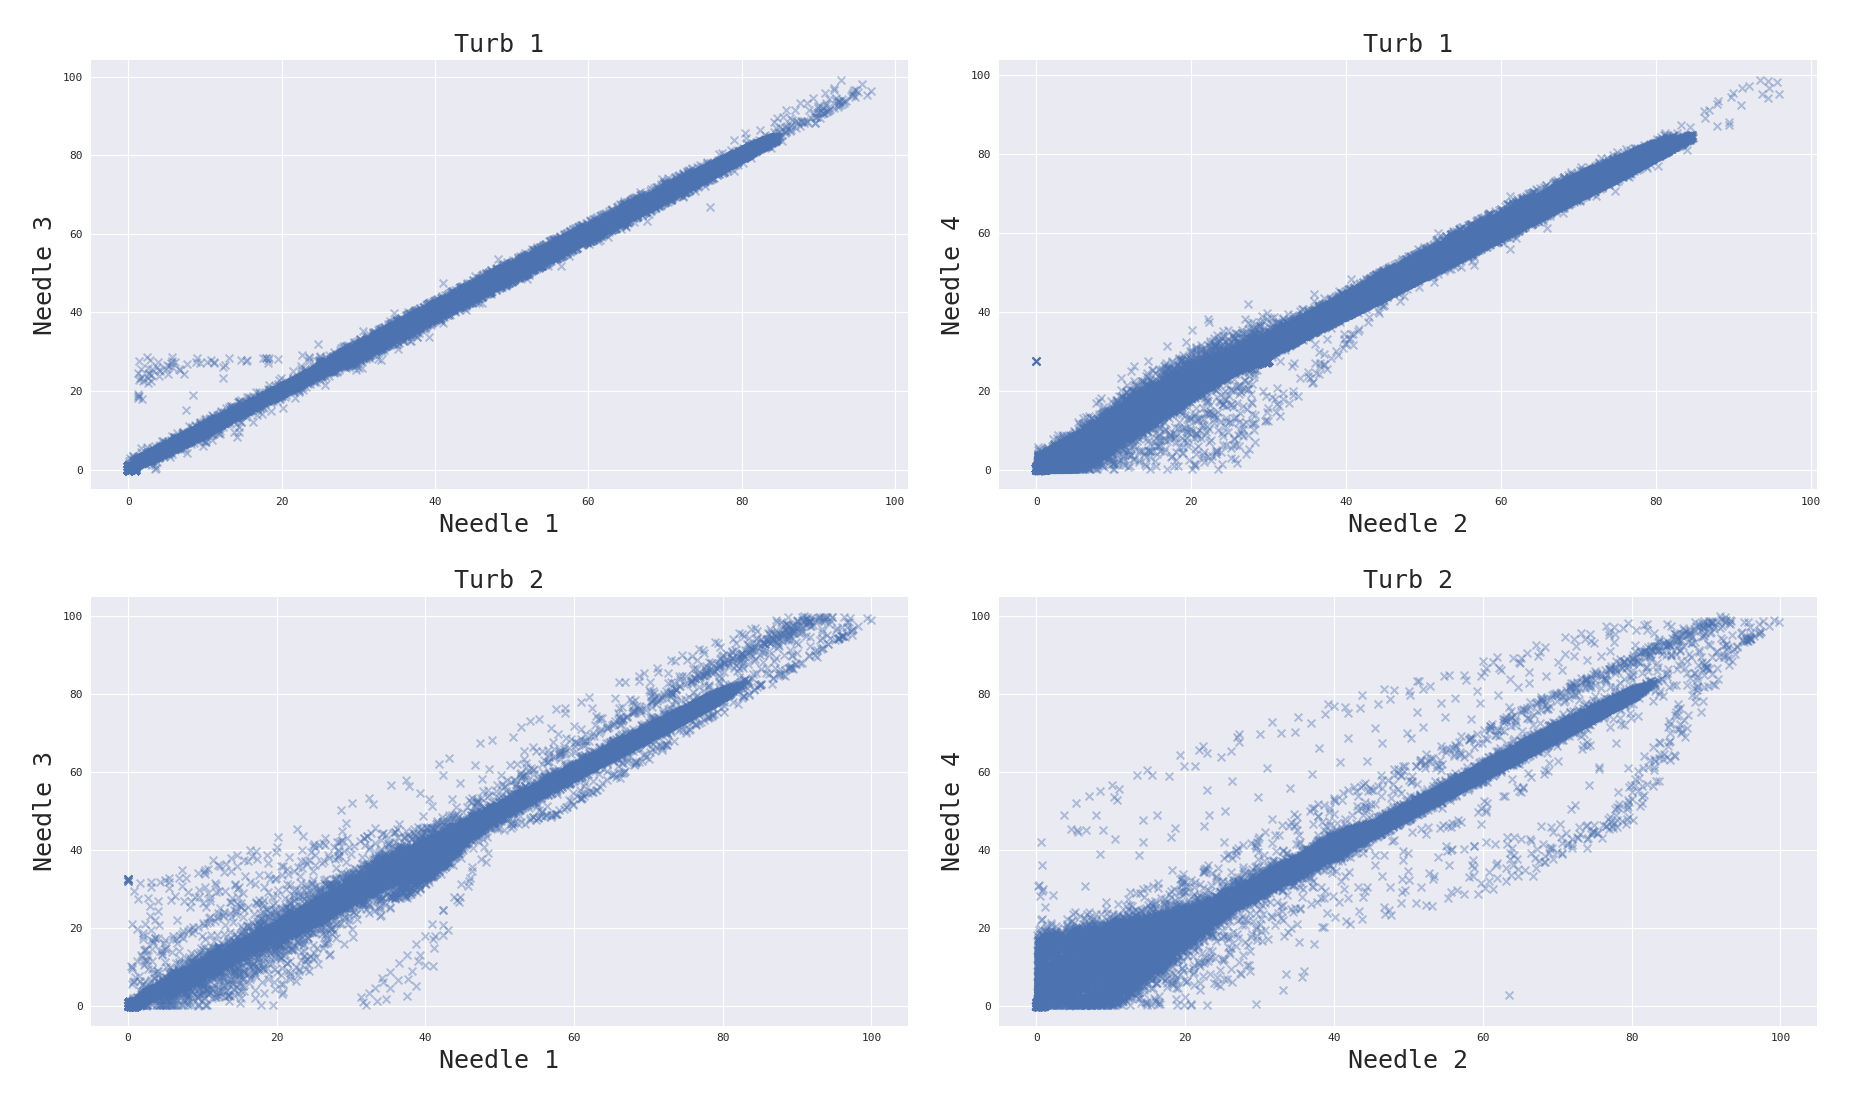
\includegraphics[width=\textwidth]{report/figures/data/plant1_needles.png}
            \caption{Pairwise operated needles for plant 1}
            \label{fig:plant1_needles}
        \end{figure}
        % Figure \ref{fig:n_pos_0203} to \ref{fig:n_pos_aft_0303} shows the needle positions for two dates surrounding the reported incident, and all data after. Figure \ref{fig:n_pos_aft_0303} show that the problem was fixed when reported in early March. Figure \ref{fig:n_pos_0203} and \ref{fig:n_pos_0303} shows the two days with worst performance, and one can see that many of the worst data-points from the lower right plot in figure \ref{fig:plant1_needles}, looks to be the same as the ones shown in figure \ref{fig:n_pos_0203} and \ref{fig:n_pos_0303}.
        
        Figure \ref{fig:plan1_scatter_20161001-20170304} shows a scatter plot of the needles [2,4] for the last 150 days up to the reported incident. The sample color changes as days goes by, as seen in the color bar. It becomes clear that the most deviating samples are from the days around the incident. There are very few dark samples that deviate from the linear pattern, indicating normal system operation 150 days before the incident. Figure \ref{fig:plan1_scatter_20161001-20170304_40} shows the same plot zoomed in. Looking at the bottom left corner of the plot, one can see that needle 4 is lagging behind needle 2. It is also clear that the lagg is worsening with time, as the color is shifting from dark to yellow. What happens the day of the incident is hard to explain, and the data takes on a completely new pattern. Unfortunately it was not possible to get the full information from the energy company about what maintenance was performed to fix this problem. It is therefore assumed that the incident is a result of the system degradation seen leading up to 02.03.2017. Hence this can be used to detect system degradation before the performance become unacceptable.     
        \begin{figure}
            \centering
            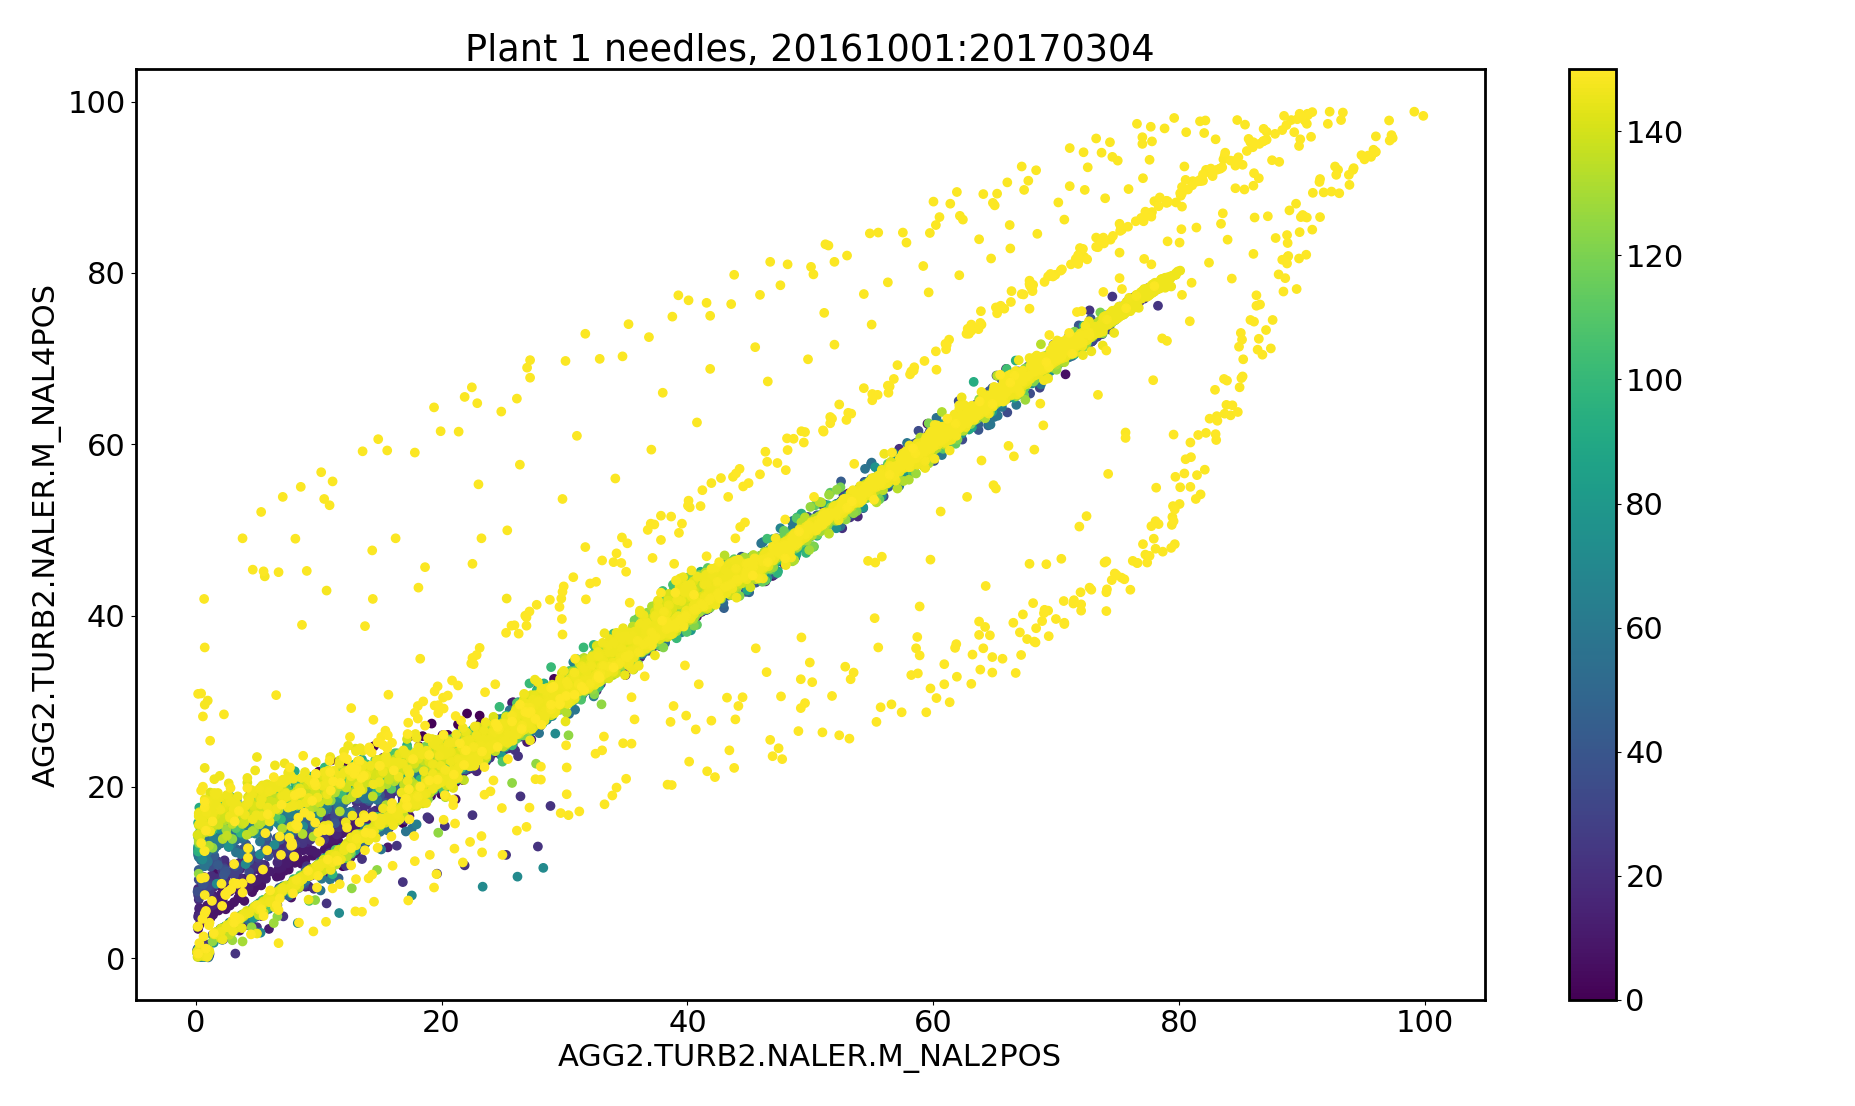
\includegraphics[width=\textwidth]{report/figures/analysis/plant1_error/needle_2_4_20161001-20170304_dots.png}
            \caption{Turbine 2 needle [2,4] scatterplot of the 150 days leading up to the incident.}
            \label{fig:plan1_scatter_20161001-20170304}
        \end{figure}
        
        \begin{figure}
            \centering
            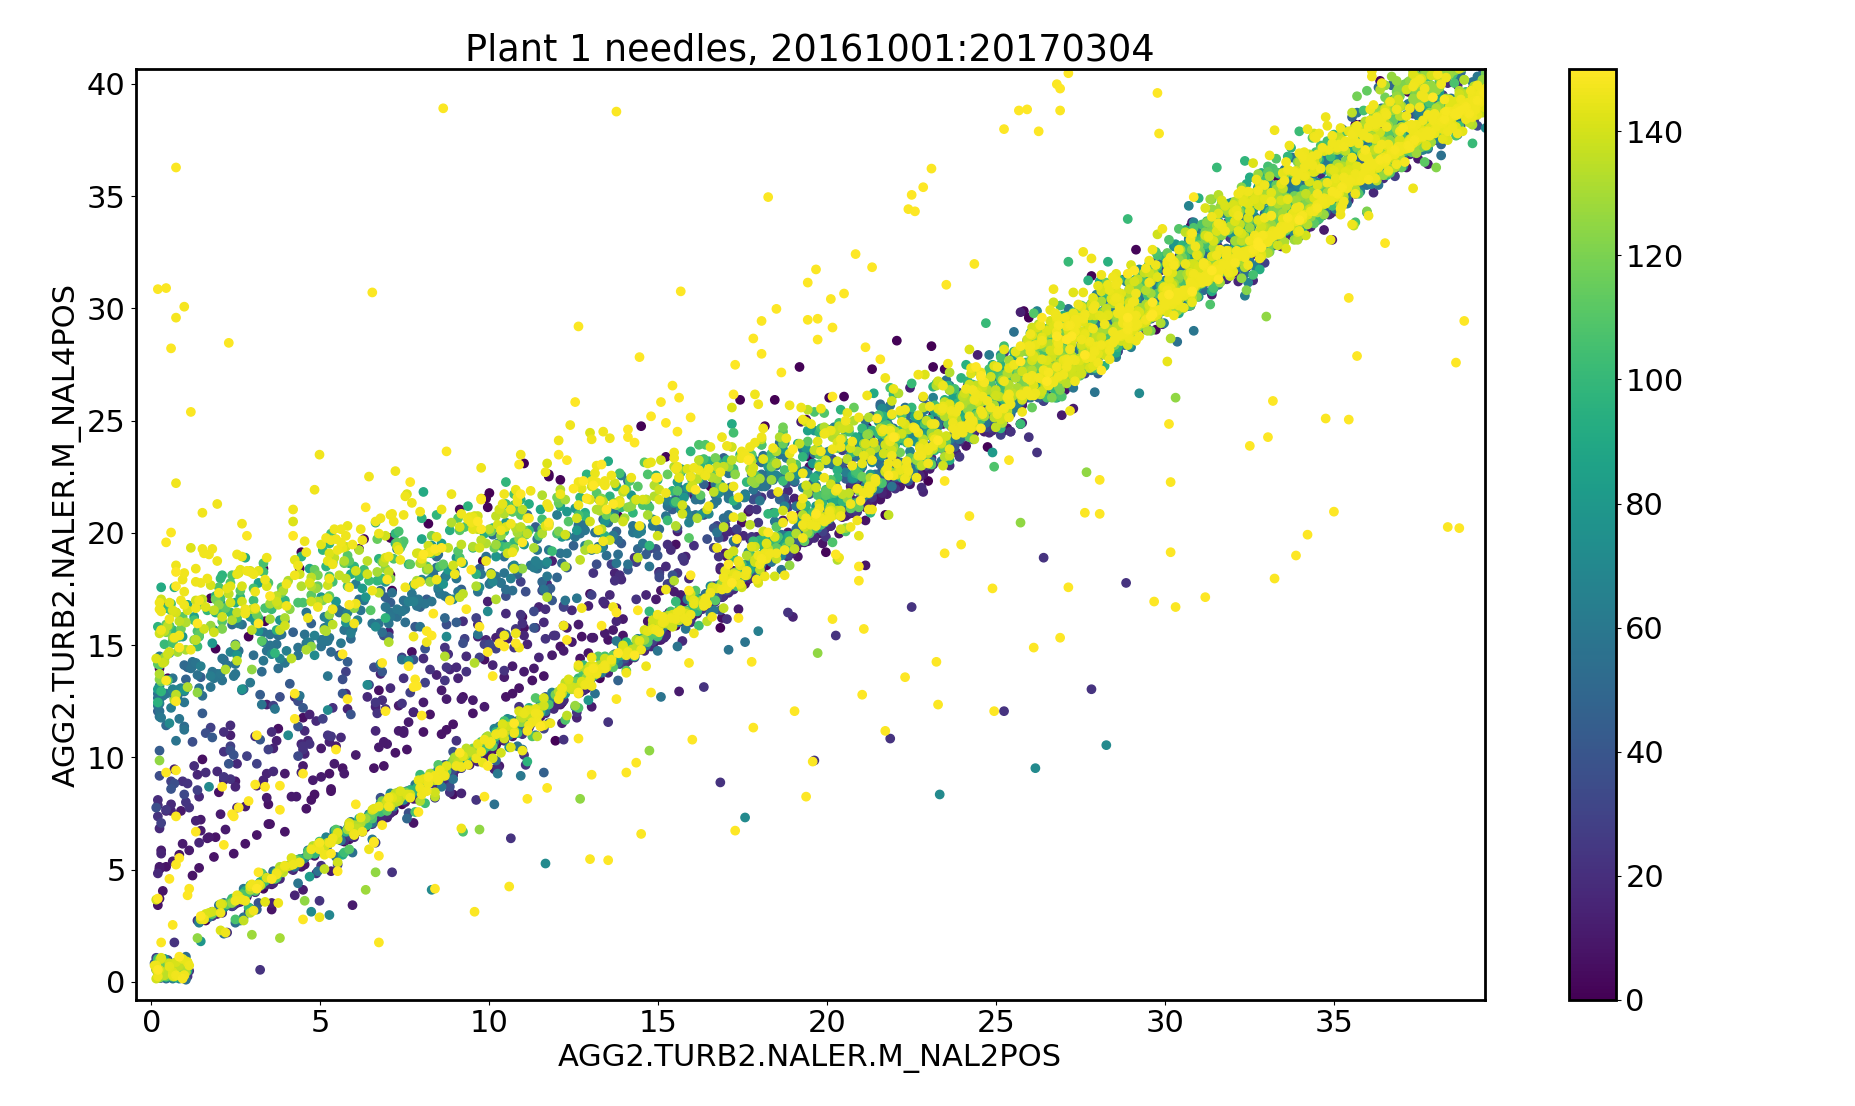
\includegraphics[width=\textwidth]{report/figures/analysis/plant1_error/needle_2_4_20161001-20170304_40_dots.png}
            \caption{Turbine 2 needle [2,4] scatterplot of the 150 days leading up to the incident zoomed in.}
            \label{fig:plan1_scatter_20161001-20170304_40}
        \end{figure}
        
        % \begin{figure}[h!]
        %     \caption*{Turbine 2 needle positions}
        %     \begin{minipage}[b]{0.5\linewidth}
        %         \centering
        %         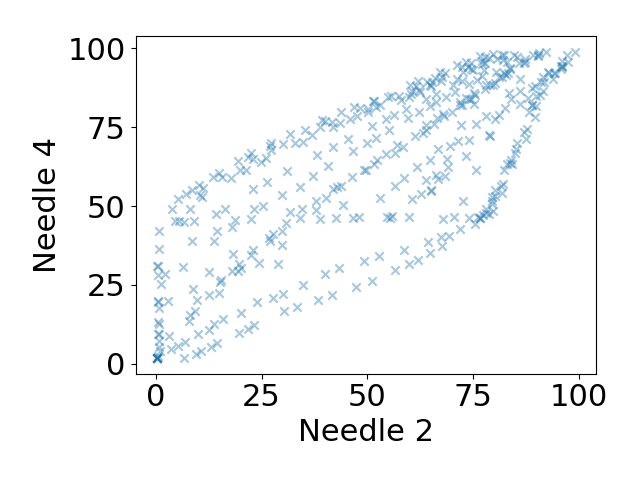
\includegraphics[width = \textwidth]{report/figures/data/turb2_n2_n4_02032017.png}
        %         \caption{02.03.2017}
        %         \label{fig:n_pos_0203}
        %     \end{minipage}
        %     \begin{minipage}[b]{0.5\linewidth}
        %         \centering
        %         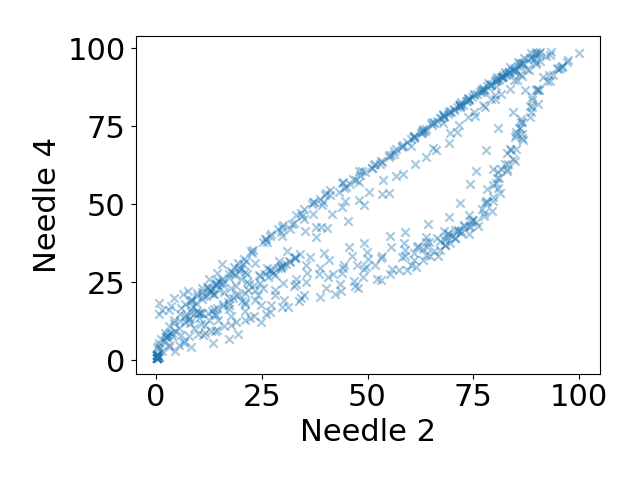
\includegraphics[width = \textwidth]{report/figures/data/turb2_n2_n4_03032017.png}
        %         \caption{03.03.2017}
        %         \label{fig:n_pos_0303}
        %     \end{minipage}
        %     \begin{minipage}[b]{0.5\linewidth}
        %         \centering
        %         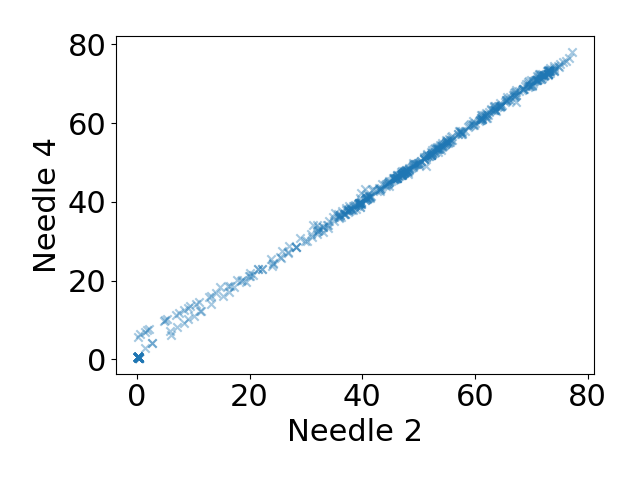
\includegraphics[width = \textwidth]{report/figures/data/turb2_n2_n4_after_04032017.png}
        %         \caption{04.03.2017 ->}
        %         \label{fig:n_pos_aft_0303}
        %     \end{minipage}
        % \end{figure}
        
        To investigate how the turbine had performed earlier in the sampling period, figure \ref{fig:plant1_needle_error} was created. It shows the needles positions on top of each other, and the error between them. The reported incident $02.03.2017$ can clearly be seen in the plot. The claim made earlier that the system is gradually degrading can be supported by the growing error up to the incident. Interestingly, there also seem to have been som issues with the operation in both 2014 and 2016. There is however no reported incidents in the plant log. 
        \begin{figure}
            \centering
            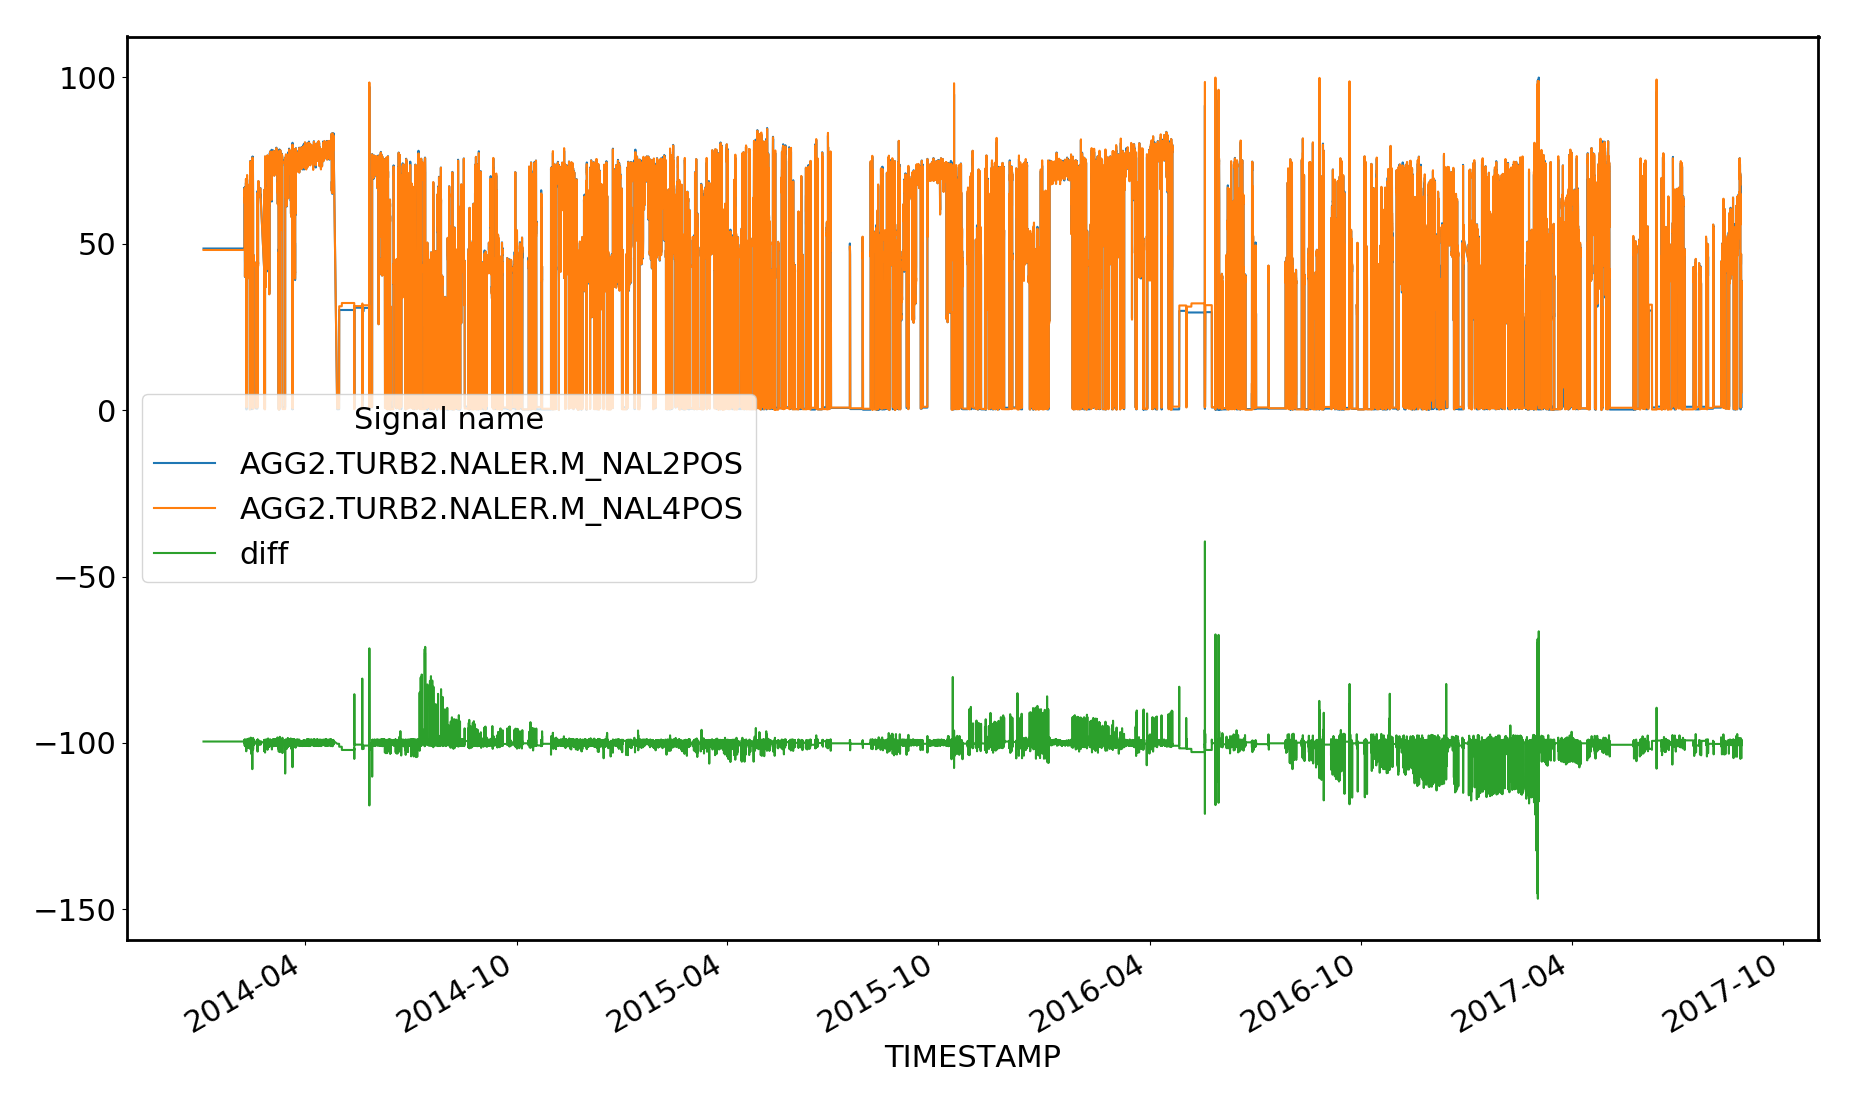
\includegraphics[width=\textwidth]{report/figures/data/turbine2_needle2_4.png}
            \caption{Overview of needle error for turbine 2, needle [2,4] on plan 1}
            \label{fig:plant1_needle_error}
        \end{figure}
        
        
    \subsection{Other Pelton needle incidents}
        The log reported two other issues with the turbine needles at plant $1$, that are observable in a scatter plot, seen in figure \ref{fig:start_failure_turb1} and \ref{fig:start_failure_turb2}. Both are start up failures due to problems with the needle operation. The failure on 10.12.2014 has a similar pattern as the reported incident, and can then used as an additional test on how well the anomaly detection techniques perform.
        \begin{figure}[h!]
            \caption*{Start up errors}
            \begin{minipage}[b]{0.5\linewidth}
                \centering
                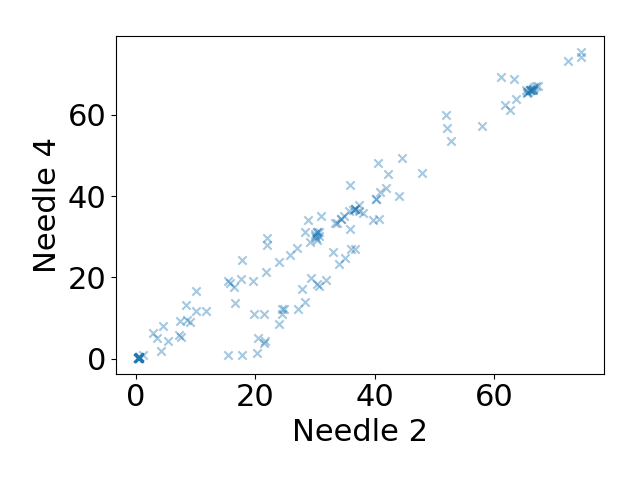
\includegraphics[width = \textwidth]{report/figures/data/turb1_n2_n4_scatter_start_failure_10122014.png}
                \caption{Turbine 1, 10.12.2014}
                \label{fig:start_failure_turb1}
            \end{minipage}
            \begin{minipage}[b]{0.5\linewidth}
                \centering
                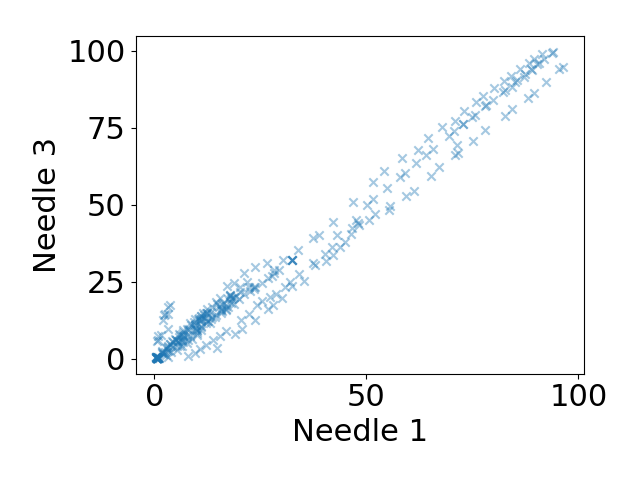
\includegraphics[width = \textwidth]{report/figures/data/turb2_n1_n3_start_failure_25082016.png}
                \caption{Turbine 2, 25.08.2016}
                \label{fig:start_failure_turb2}
            \end{minipage}
        \end{figure}
        
        
    
    \subsection{Other plants with Pelton turbines}
        Further investigation showed that the second plant with Pelton turbines also have two turbines with pairwise operated needles. The third Pelton plant only have one turbine, and the needles are not pairwise operated. The turbine use from 1 to 5 needles depending on the the produced power. Data from this plant could be used to generalize the anomaly detection methods to handle any combination of needles, but this will not be covered in this thesis. The needle operation for the second plant is seen in figure \ref{fig:plant2_needles}. One can see that turbine $1$ has no sampling on needle $1$, but the three other pairs are sampled correctly. Plant 2 further motivates that there is something wrong with the needles for plant $1$. All needle pairs follow the linear pattern much better, and have very few anomalies.
        \begin{figure}
            \centering
            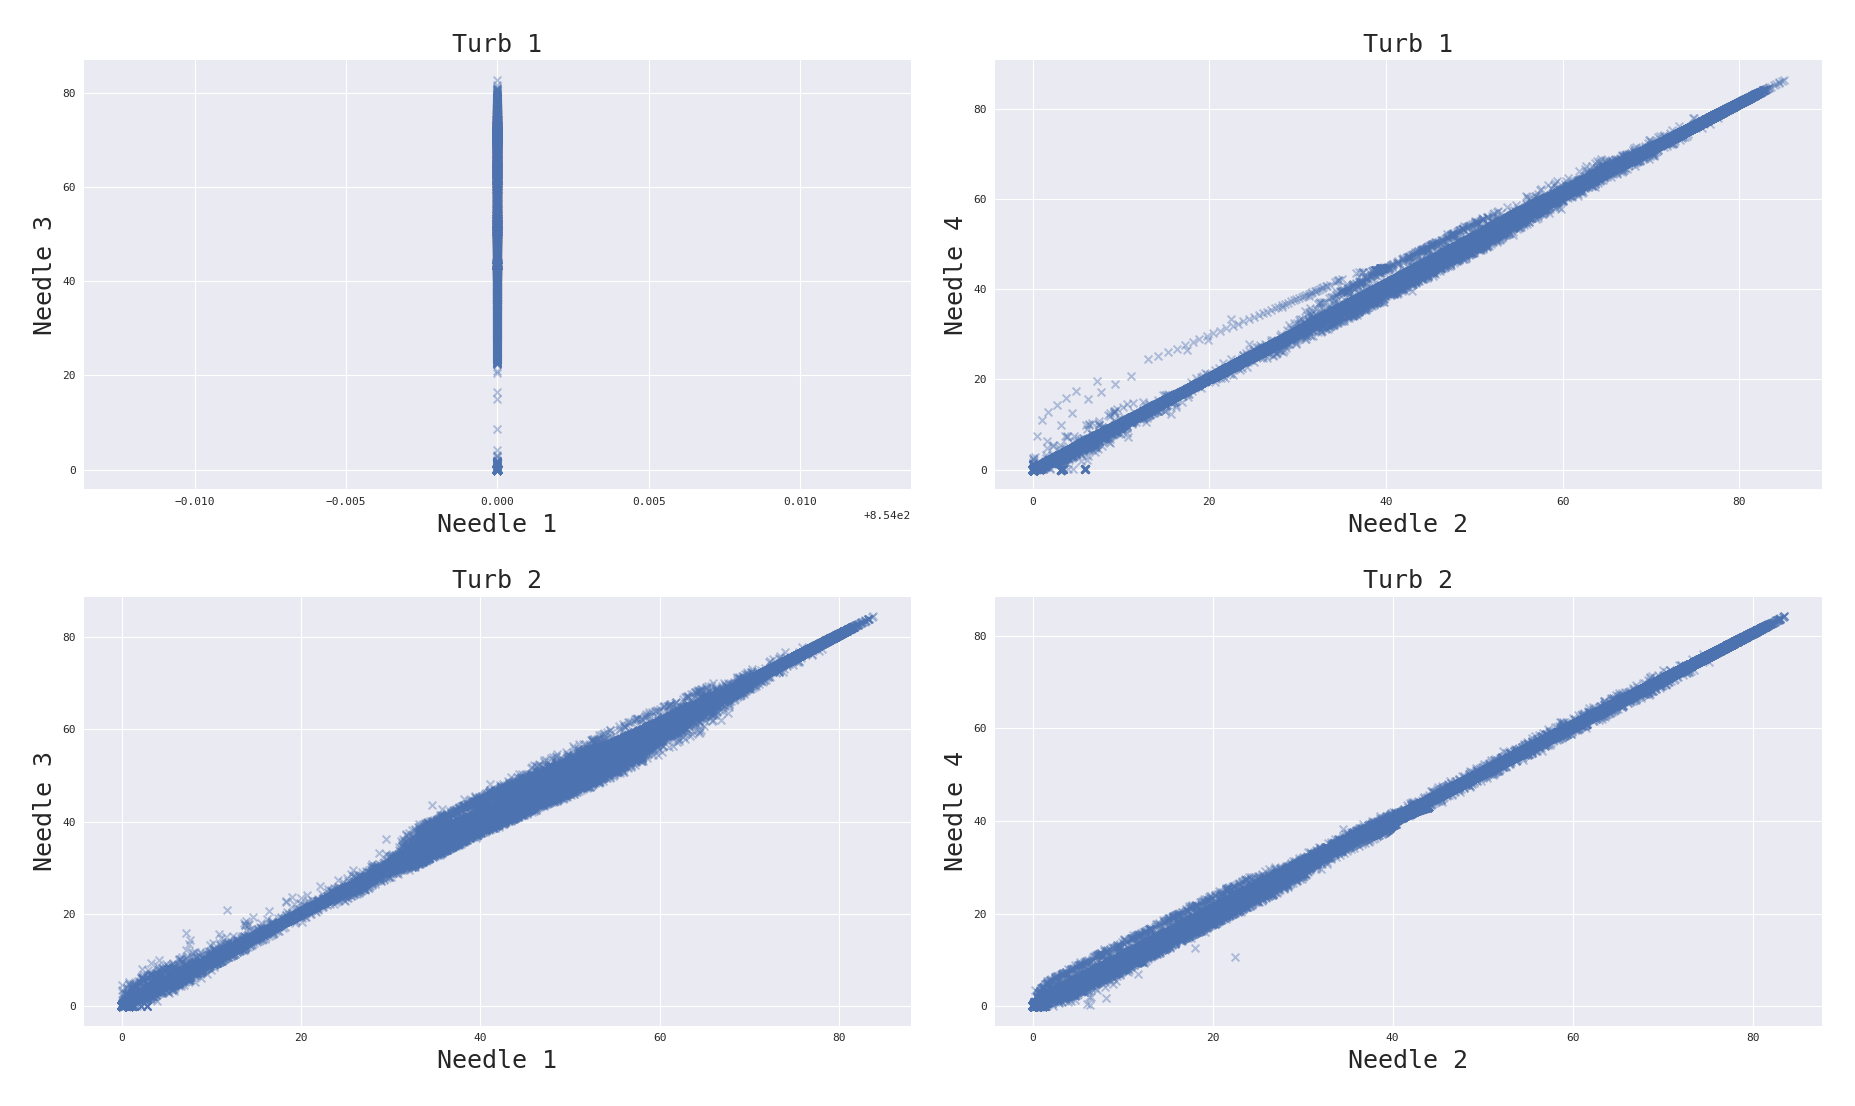
\includegraphics[width=\textwidth]{report/figures/data/plant_2_needle_plot.png}
            \caption{Pairwise operated needles for plant 2}
            \label{fig:plant2_needles}
        \end{figure}
        
        
        
    % \section{Other process signals}
        
    
        
    %     mention that this alone is a case one can build upon but to track the error to other processvariable would be very interesintg both for condition monitoring but also for identification of the fault and why it happened. 
        
        
    %     It is important to understand that an outlier in the data does not necessarily mean that something is about to break. There is a possibility that the sample is an indication of a condition change in the equipmnet, but it might also be due to error in the measurement, noise or just a deviation in the ongoing process. This makes this kind of analysis even harder, an outlier might just be a coincident, that yields little to no information. 
        
         
         
    \subsection{Artificial case}\label{subsec:arti}
        Due to not having any incidents similar to the one seen at plant 1 turbine 2, an artificial error replicating the pattern is created. The main motivation is to see when an error that is increasing over time is detectable. A subset of the data sampled at plant 2 is altered to replicate an error similar to the one seen for plant 1. By doing so, one knows exactly when the error starts occurring, this can then be used to evaluate how early different anomaly detection techniques detects anomalies.
    
        The turbine needles are controlled through a hydraulic system. A hydraulic system can suffer from many problems which can cause operational problems, such as pressure drops due to both external and internal leakage. External leakage is often broken hoses or pipes. Internal leakages are within the pumps and actuators. Both types of leakages reduce the system pressure, and can slow down the motion of the system. Oil contamination can also be an issue if filters are not maintained at a given interval, unfiltered oil can then lead to clogged components, which can lead to pressure drops. The main theory of the problems seen at plant 1 is that the oil flow is restricted in one direction. As needle 4 closes, the larger the differential pressure caused by the water head being restricted becomes. As the differential pressure grows, closing the needle requires more force. This means that if the hydraulic system is suffering from reduced capacity in one direction, the motion of the needle will slow down as the needle close. Figure \ref{fig:plant2_arti_error} shows the colored scatter plot for the plant 2 data with and without the artificial error. As can be seen it has a similar pattern to what was seen at plant 1 in the days leading up to the reported incident. Figure \ref{fig:plant2_arti_error_40}, shows a close up on the lower openings of the needle. The deviation between the two needles increase with time, as seen in the case with plant 1. The artificial error is added to data sampled from needle pair [2,4] on turbine 2 at plant 2. Data from 20161001 to 20170401 is used, and the artificial error is added from 20170201.     
        
        \begin{figure}
            \begin{minipage}[b]{0.5\linewidth}
                \centering
                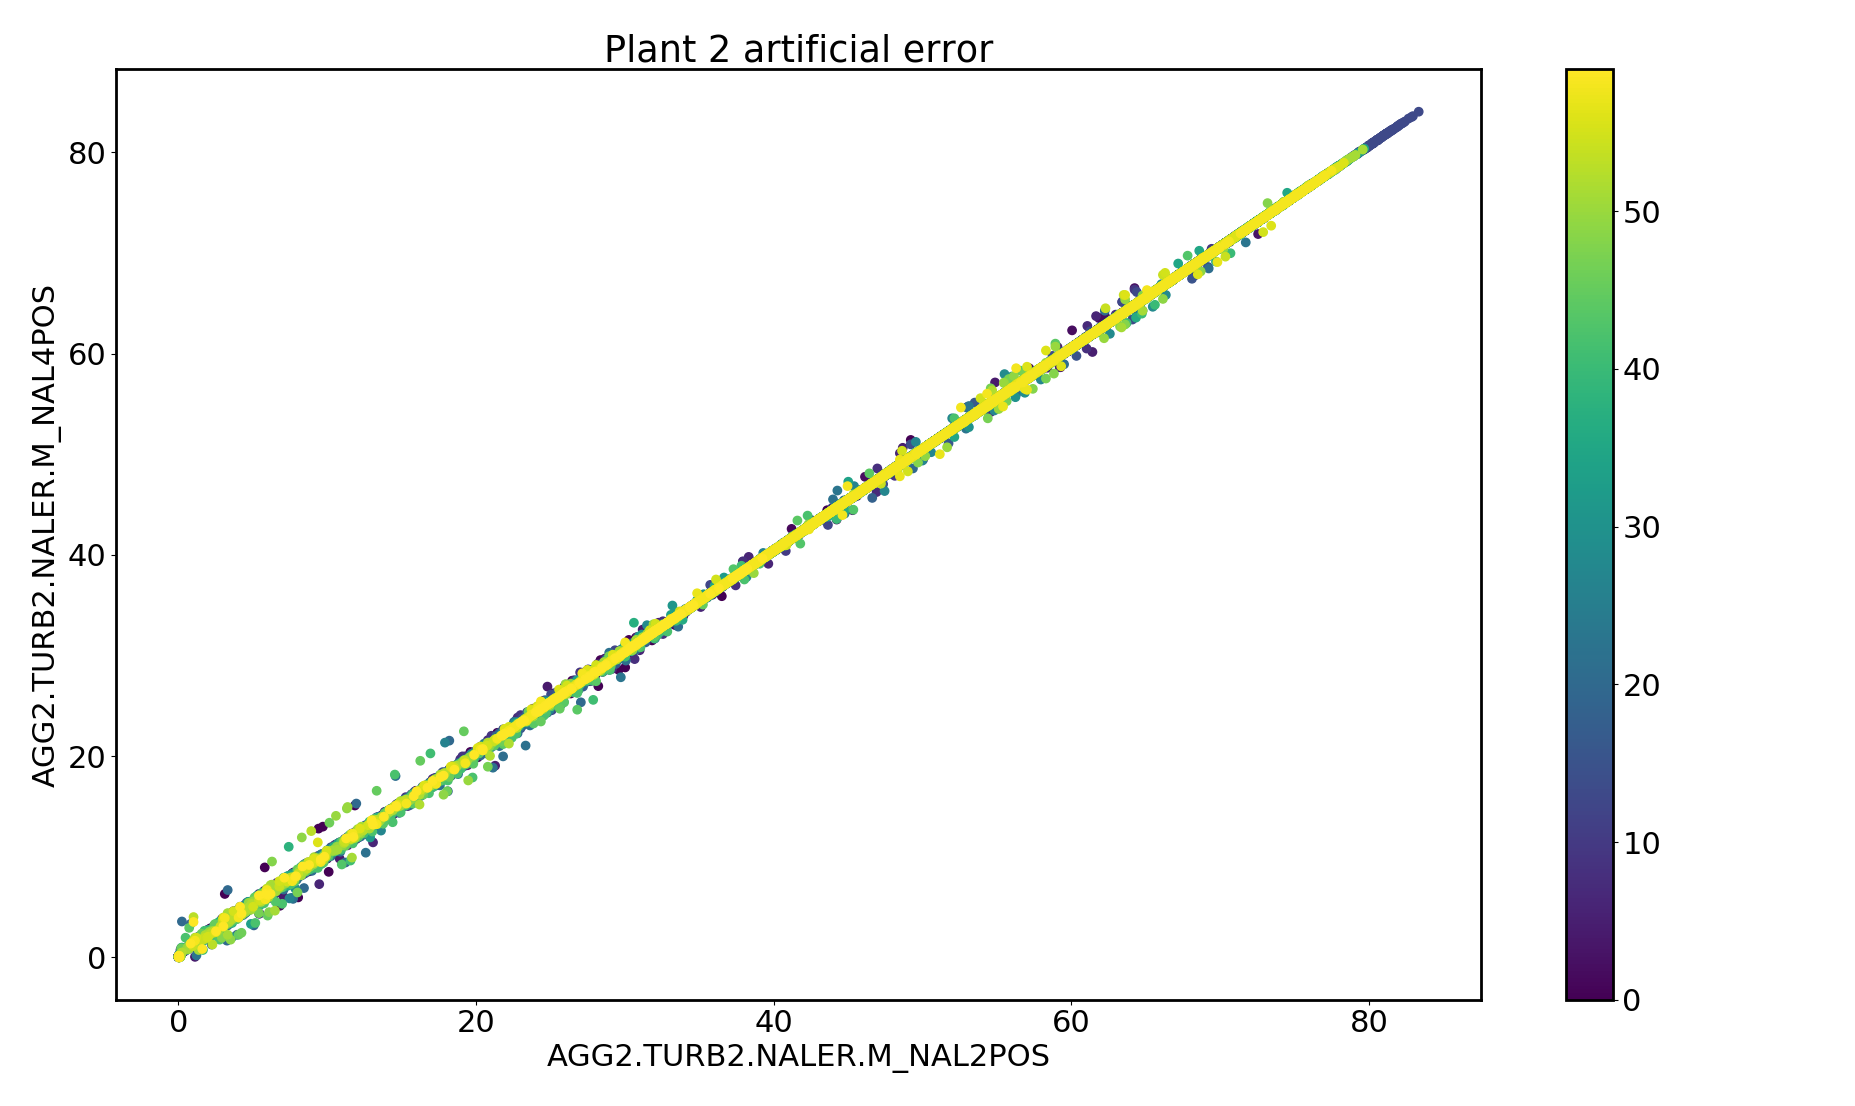
\includegraphics[width = \textwidth]{report/figures/analysis/artificial error/original_data.png}
                % \caption{Original data}
                % \label{fig:plant2_arti_orig}
            \end{minipage}
            \begin{minipage}[b]{0.5\linewidth}
                \centering
                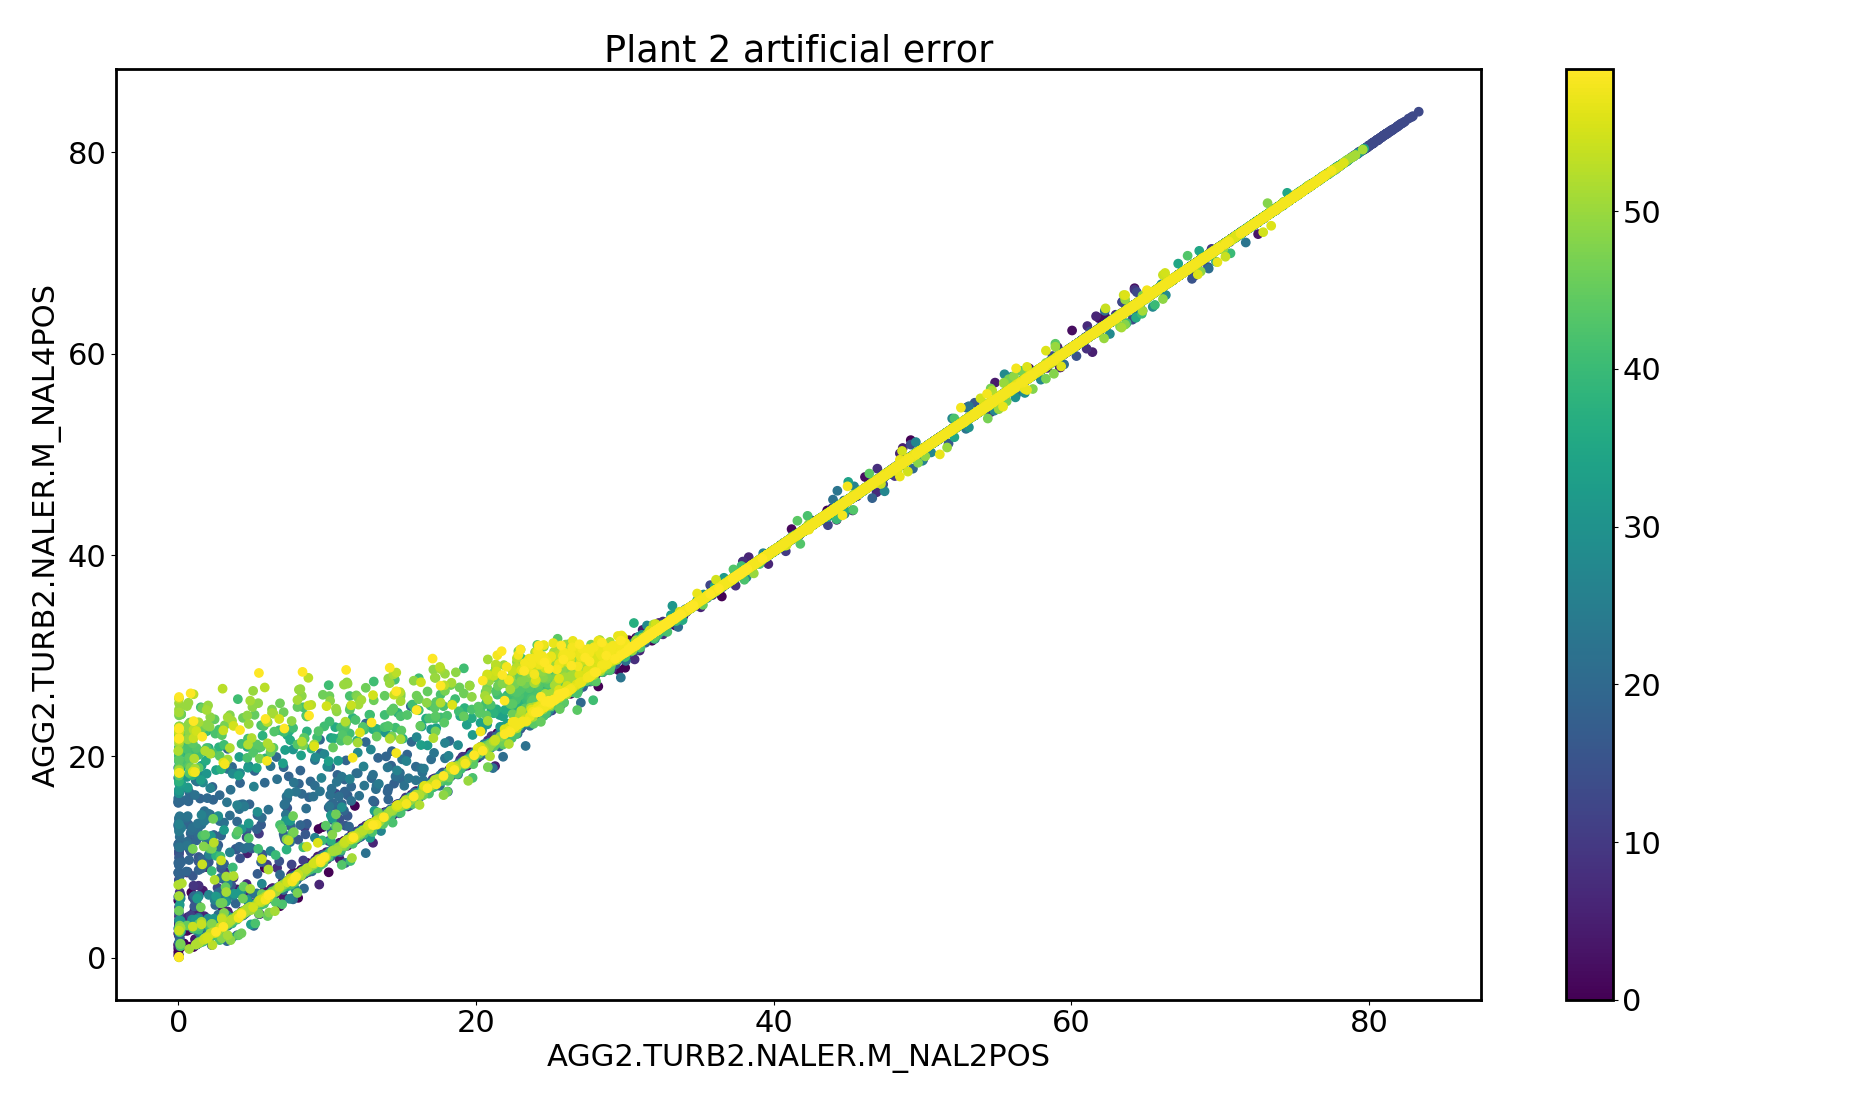
\includegraphics[width = \textwidth]{report/figures/analysis/artificial error/plant2_artificial_error_scatter_colored.png}
                % \caption{Added artificial error}
                % \label{fig:plant2_arti_error}
            \end{minipage}
            \caption{Colored scatter plot of the data before and after adding the artificial error}
            \label{fig:plant2_arti_error}
        \end{figure}
        
        \begin{figure}
            \centering
            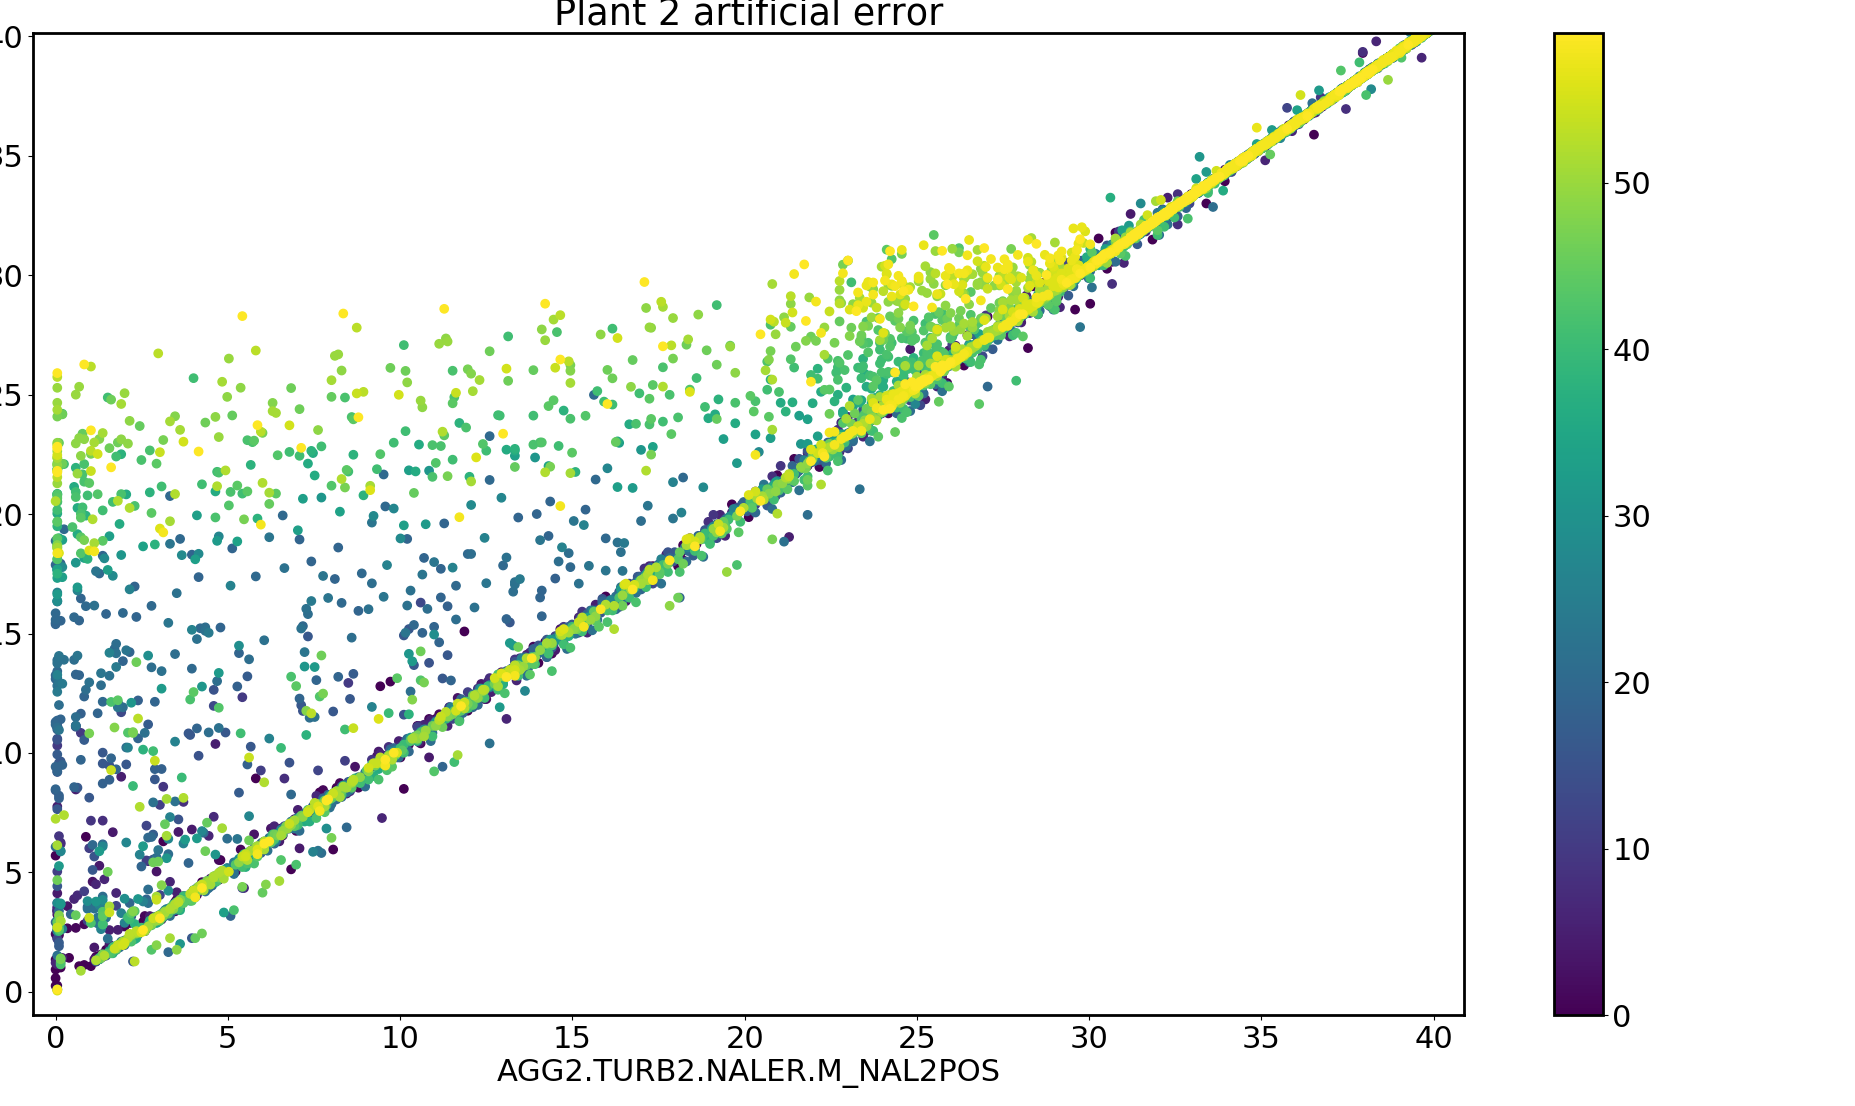
\includegraphics[width = \textwidth]{report/figures/analysis/artificial error/plant2_artificial_error_scatter_colored_40.png}
            \caption{Caption}
            \label{fig:plant2_arti_error_40}
        \end{figure}